%%%%%%%%%%%%%%%%%%%%%%%%%%%%%%%%%%%%%%%%%
% Beamer Presentation
% LaTeX Template
% Version 1.0 (10/11/12)
%
% This template has been downloaded from:
% http://www.LaTeXTemplates.com
%
% License:
% CC BY-NC-SA 3.0 (http://creativecommons.org/licenses/by-nc-sa/3.0/)
%
%%%%%%%%%%%%%%%%%%%%%%%%%%%%%%%%%%%%%%%%%

%----------------------------------------------------------------------------------------
%	PACKAGES AND THEMES
%----------------------------------------------------------------------------------------

\documentclass{beamer}

\mode<presentation> {

% The Beamer class comes with a number of default slide themes
% which change the colors and layouts of slides. Below this is a list
% of all the themes, uncomment each in turn to see what they look like.

\usetheme{default}
%\usetheme{AnnArbor}
%\usetheme{Antibes}
%\usetheme{Bergen}
%\usetheme{Berkeley}
%\usetheme{Berlin}
%\usetheme{Boadilla}
%\usetheme{CambridgeUS}
%\usetheme{Copenhagen}
%\usetheme{Darmstadt}
%\usetheme{Dresden}
%\usetheme{Frankfurt}
%\usetheme{Goettingen}
%\usetheme{Hannover}
%\usetheme{Ilmenau}
%\usetheme{JuanLesPins}
%\usetheme{Luebeck}
%\usetheme{Madrid}
%\usetheme{Malmoe}
%\usetheme{Marburg}
%\usetheme{Montpellier}
%\usetheme{PaloAlto}
%\usetheme{Pittsburgh}
%\usetheme{Rochester}
%\usetheme{Singapore}
%\usetheme{Szeged}
%\usetheme{Warsaw}

% As well as themes, the Beamer class has a number of color themes
% for any slide theme. Uncomment each of these in turn to see how it
% changes the colors of your current slide theme.

%\usecolortheme{albatross}
%\usecolortheme{beaver}
%\usecolortheme{beetle}
%\usecolortheme{crane}
%\usecolortheme{dolphin}
%\usecolortheme{dove}
%\usecolortheme{fly}
%\usecolortheme{lily}
%\usecolortheme{orchid}
%\usecolortheme{rose}
%\usecolortheme{seagull}
%\usecolortheme{seahorse}
%\usecolortheme{whale}
%\usecolortheme{wolverine}

\usepackage[official]{eurosym}
\usepackage{svg}
\usepackage{amsmath}
\usepackage{graphicx}
\usepackage{multirow}
\usepackage[utf8]{inputenc}
\usepackage{subfig}
%\setbeamertemplate{footline} % To remove the footer line in all slides uncomment this line
%\setbeamertemplate{footline}[page number] % To replace the footer line in all slides with a simple slide count uncomment this line

%\setbeamertemplate{navigation symbols}{} % To remove the navigation symbols from the bottom of all slides uncomment this line
}

\usepackage{graphicx} % Allows including images
\usepackage{booktabs} % Allows the use of \toprule, \midrule and \bottomrule in tables

%----------------------------------------------------------------------------------------
%	TITLE PAGE
%----------------------------------------------------------------------------------------

\title[BPP]{Bin Packing Problem:\\ A general purpose Hill Climbing procedure } % The short title appears at the bottom of every slide, the full title is only on the title page


 % Your name
\institute[FSU] % Your institution as it will appear on the bottom of every slide, may be shorthand to save space
{ 
Seminar Modern Heuristics \\
Dr. Rico Walter
}

\author{Lukas Schmauch, Sebsatian Wolf}
\date{Februar 2021} % Date, can be changed to a custom date

\begin{document}
\begin{frame}
\titlepage % Print the title page as the first slide
\end{frame}
%-------------------------------------
\begin{frame}
\frametitle{Übersicht} 
\tableofcontents
\section{Was ist das Bin Packing Problem?} 
\section{Computational Studies}
\section{Zusammenfassung} 
\end{frame}

%----------------------------------------------------------------------------------------
%	PRESENTATION SLIDES
%----------------------------------------------------------------------------------------
\begin{frame}

\frametitle{Verteilungsfunktion}

\begin{footnotesize}
\begin{equation}
mit \ r = \frac{Z_{HC}-LB}{LB} * 100\%
\end{equation}
\end{footnotesize}

\begin{figure}[!htbp]
\begin{center}
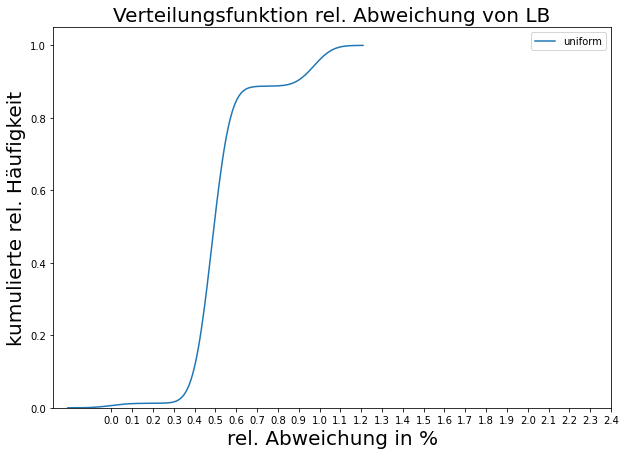
\includegraphics[scale=0.3]{img/dist.png}
\end{center}
\caption{rel. Abweichung von LB nach 10 Sec.}
\label{fig:architecture}
\end{figure}



\end{frame}
%----------------------------------------------------------------------------------------
\begin{frame}

\frametitle{Verteilungsfunktion}

\begin{footnotesize}
\begin{equation}
mit \ r = \frac{Z_{HC}-LB}{LB} * 100\%
\end{equation}
\end{footnotesize}

\begin{figure}[!htbp]
\begin{center}
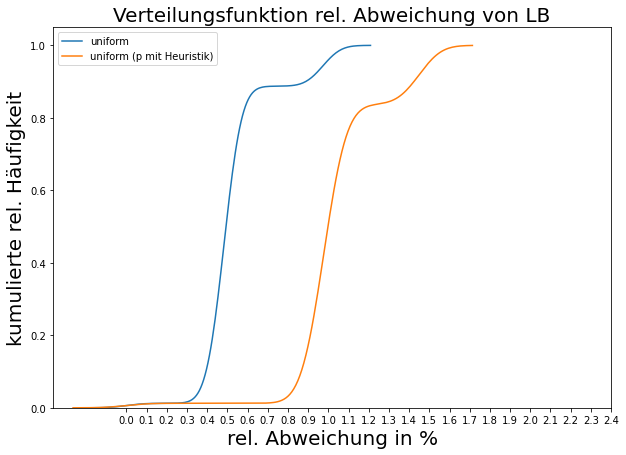
\includegraphics[scale=0.3]{img/dist2.png}
\end{center}
\caption{rel. Abweichung von LB nach 10 Sec.}
\label{fig:architecture}
\end{figure}



\end{frame}

%----------------------------------------------------------------------------------------
\begin{frame}

\frametitle{Optimalitätsanalyse Instanzgruppe Uniform}
\begin{footnotesize}
\begin{equation}
L_1 = \left\lceil\sum_{j=1}^{n} \frac{w_j}{C}\right\rceil
\end{equation}
\end{footnotesize}


\begin{figure}[!htbp]
\begin{center}
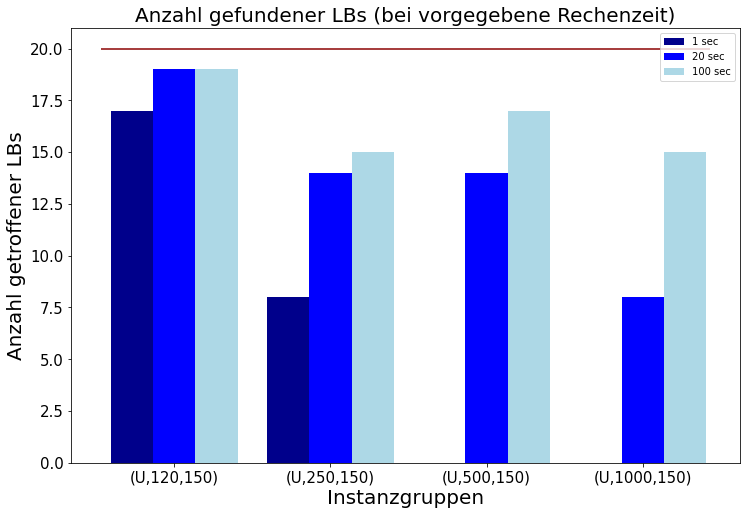
\includegraphics[scale=0.3]{img/lb_unif.png}
\end{center}
\caption{Anzahl gefundener LBs}
\label{fig:architecture}
\end{figure}



\end{frame}
%----------------------------------------------------------------------------------------
\begin{frame}

\frametitle{Optimalitätsanalyse Instanzgruppe Uniform}

\begin{figure}[!htbp]
\begin{center}
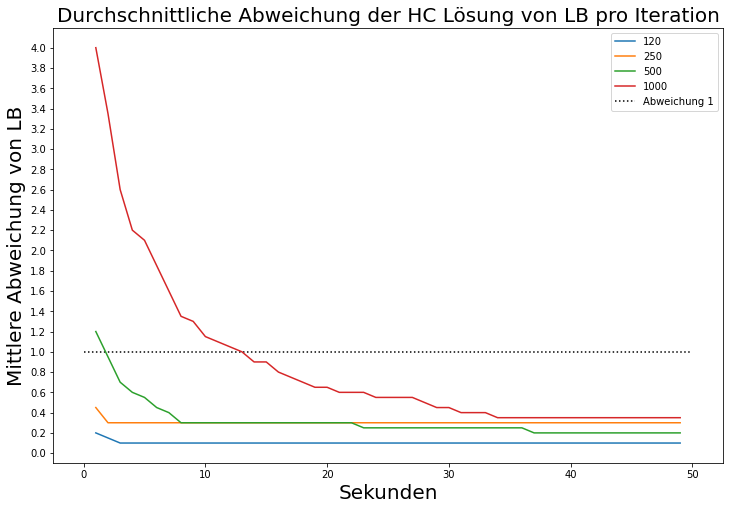
\includegraphics[scale=0.3]{img/uniform_time.png}
\end{center}
\caption{Mittlere Abweichung von LB pro Zeiteinheit}
\label{fig:architecture}
\end{figure}



\end{frame}


%----------------------------------------------------------------------------------------
\begin{frame}
\frametitle{Vergleich mit anderer Permutationswahl}


\begin{columns}[c] % The "c" option specifies centered vertical alignment while the "t" option is used for top vertical alignment

\column{.5\textwidth} % Left column and width
\begin{figure}[!htbp]
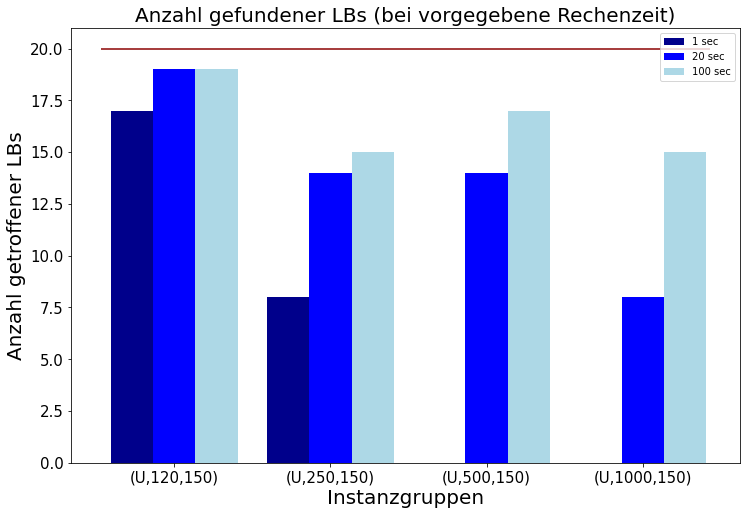
\includegraphics[scale=0.2]{img/lb_unif.png}
\caption{Random Permutation}
\label{fig:architecture}
\end{figure}


\column{.5\textwidth} % Right column and width
\begin{figure}[!htbp]
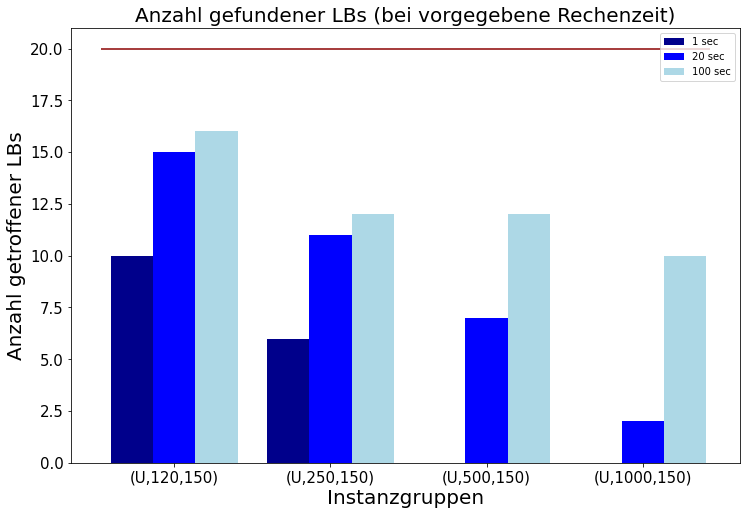
\includegraphics[scale=0.2]{img/lb_unif_heuristic.png}
\caption{Minimale Itemzahl}
\label{fig:architecture}
\end{figure}


\end{columns}
\end{frame}
%%----------------------------------------------------------------------------------------
%\begin{frame}
%\frametitle{Warum CNNs statt klassischer Neuronaler Netze?}
%\begin{figure}[!htbp]
%\begin{center}
%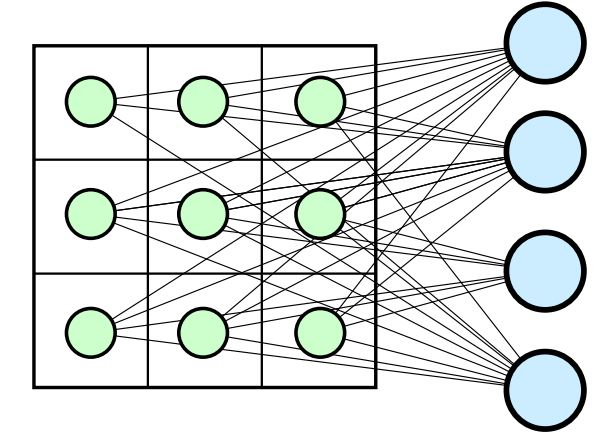
\includegraphics[scale=0.3]{img/mlp.jpg}
%\end{center}
%\caption{Ausschnitt erste Schicht eines MLPs mit Bilddaten \cite{3}}
%\label{fig:architecture}
%\end{figure}
%
%
%\begin{footnotesize}
%\begin{itemize}
%\item Annahme: Eingabe sei Grauwertbild mit \textbf{1 Megapixel} (1024x1024x1),\\ ein verborgener Layer mit \textbf{k Knoten}
%\item Anzahl der \textbf{zu schätzenden Parameter} der ersten Schicht:  $1024 \cdot 1024 \cdot 1 \cdot k \approx k$ \textbf{Millionen Parameter (Overfitting!!!)}
%\item \textbf{Herausforderung CNN:} drastische Reduktion der Parameter bei gleichzeitger Invarianz ggü. Verschiebungen
%\end{itemize}
%\end{footnotesize}
%
%
%\end{frame}
%%----------------------------------------------------------------------------------------
%
%%----------------------------------------------------------------------------------------
%\begin{frame}
%
%\frametitle{Architektur eines CNNs}
%\begin{footnotesize}
%\begin{itemize}
%\item \textbf{Detection Stage:} Convolutional Layer + ReLU, Pooling Layer
%\item \textbf{Classification Stage:} Fully Connected Layer
%\end{itemize}
%\end{footnotesize}
%\begin{figure}[!htbp]
%\begin{center}
%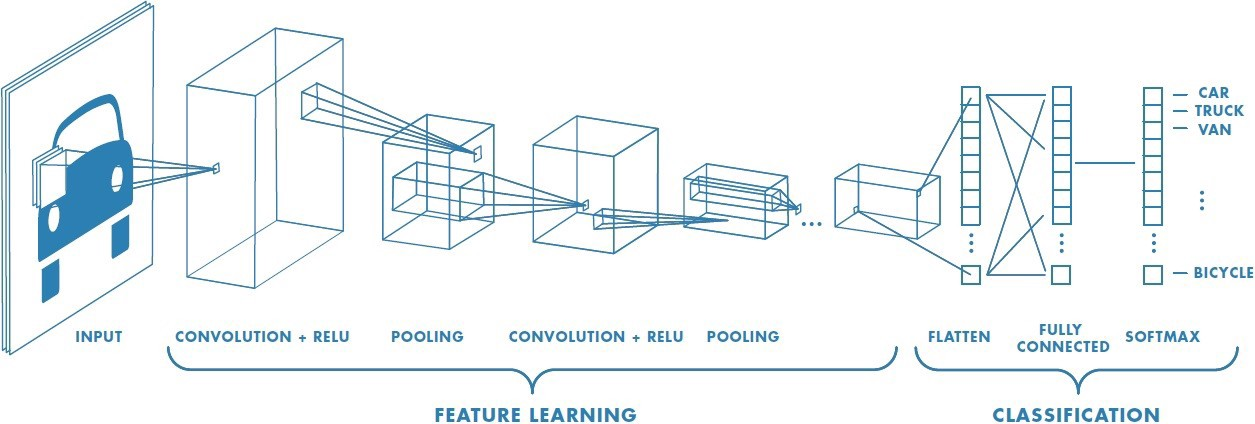
\includegraphics[scale=0.25]{img/architec2.jpeg}
%\end{center}
%\caption{Architektur eines Convolutional Neural Networks \cite{4}}
%\label{fig:architecture}
%\end{figure}
%
%
%\end{frame}
%%---------------------------------------
%\begin{frame}
%
%\frametitle{Faltungsoperation (Convolution)}
%
%\begin{footnotesize}
%\begin{itemize}
%\item \textbf{Faltung} mit einer \textbf{3x3 Faltungsmatrix} als elementweise Multiplikation und Addition \textbf{(Skalarprodukt)}
%\item Filter \textbf{gleitet schrittweise} über komplettes Eingabebild
%\item Resultierender \textbf{Pixelwert nach Maskenoperation} im gelben Bereich: 
%\begin{tiny}
%$(1\cdot1+2\cdot0+1\cdot1+2\cdot0+0\cdot1+0\cdot0+1\cdot1+0\cdot0+2\cdot1 = 5)$
%\end{tiny}
%
%\end{itemize}
%\end{footnotesize}
%
%\begin{figure}[!htbp]
%\begin{center}
%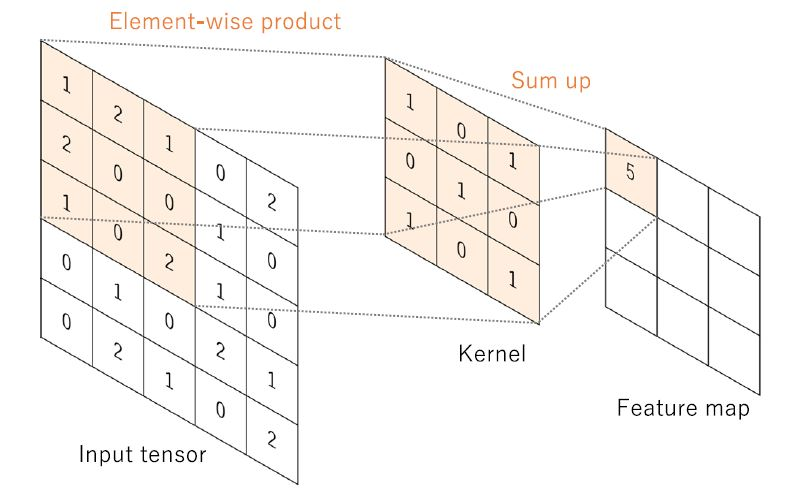
\includegraphics[scale=0.4]{img/kernel1.jpg}
%\end{center}
%
%\caption{Anwendung eines Filters bzw. Kernels auf den Input-Tensor und entstehende Feature Map \cite{2}} 
%
%
%\label{fig:kernel}
%\end{figure}
%
%
%
%\end{frame}
%%---------------------------------------
%\begin{frame}
%
%\frametitle{Einfache Kantenfilter}
%\begin{figure}
%\begin{center}
%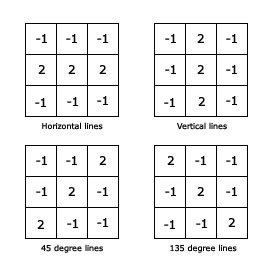
\includegraphics[scale=0.31]{img/edges.jpg}
%\end{center}
%\caption{Verschiedene Kernelgewichte, zur Extraktion der jeweiligen Kantenformen \cite{5}}
%\label{fig:kernelWeights}
%\end{figure}
%
%\begin{figure}
%\begin{center}
%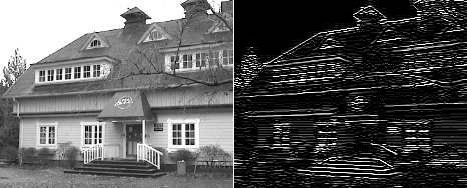
\includegraphics[scale=0.2]{img/convHouseHorizontal.jpg}
%\end{center}
%\caption{Anwendung eines horizontalen Katendetektors \cite{5}}
%\label{fig:houseH}
%\end{figure}
%\begin{scriptsize}
%\begin{itemize}
%\item \textbf{bekannte Filter:} Sobel-Operator, Laplace-Filter, Scharr-Operator, Prewitt-Operator, Roberts-Operator, Kirsch-Operator,...
%\end{itemize}
%\end{scriptsize}
%
%
%
%
%
%\end{frame}
%%---------------------------------------
%\begin{frame}
%
%\frametitle{Zusammenfassung}
%\begin{scriptsize}
%\begin{enumerate}
%\item CNNs (Faltungsnetzwerke) sind spezielle Neuronale Netze mit \textbf{mindestens einer Faltungsoperation}, statt der generellen Matrizenmultiplikation.
%\item Seit der Entwicklung \textbf{moderner Hardware (GPUs), sowie der Sammlung und Etikettierung riesieger Datenmengen} sind sie erstmals effizient trainierbar.
%\item CNNs werden erfolgreich u.a. im Bereich \textbf{Bildklassifikation}, sowie der \textbf{Handschrift- und Spracherkennung} eingesetzt.
%\item Convolutional und Pooling Layer dienen der \textbf{automatischen Extraktion von Merkmalen}.
%\item Diese Komponenten können sich beliebig oft wiederholen (tiefe Netze), um \textbf{hierarchisch komplexere Merkmale} zu identifizieren.
%\item \textbf{Filter gleiten schrittweise} über ein \textbf{Eingabebild}, um \textbf{Feature Maps} mit den hervorgehobenen Mustern zu berechnen.
%\item Die \textbf{Gewichte eines Filters} werden in der Trainingsphase \textbf{automatisch gelernt (Backpropagation)} und müssen nicht händisch bestimmt werden.
%\item Die Besonderheit von CNNs sind die \textbf{geteilten Gewichte (weight-sharing)} eines Filters über das Eingabebild, sowie die \textbf{Invarianz gegenüber Verschiebungen der Eingabe}. (Idee: Muster können sich überall im Bild befinden)
%\item Die eigentliche \textbf{Klassifikation der extrahierten Merkmale} findet in den letzen Schichten \textbf{(Fully Conneted Layer)} statt.
%\end{enumerate}
%\end{scriptsize}
%
%
%\end{frame}
%---------------------------------------

%---------------------------------------

%---------------------------------------
%\begin{frame}
%\frametitle{Der Datensatz}
%\begin{columns}[c] % The "c" option specifies centered vertical alignment while the "t" option is used for top vertical alignment
%
%\column{.3\textwidth} % Left column and width
%\begin{footnotesize}
%\begin{itemize}
%\item 64854 Einträge
%\item 50:50 Train/ Test 
%\item 38 Merkmale
%\item 20 numerisch
%\item 18 kategorisch
%\end{itemize}
%\end{footnotesize}
%
%\column{.5\textwidth} % Right column and width
%%\begin{figure}
%%\begin{center}
%%\includegraphics[width=1.0\textwidth]{pdf/distTrainTest.pdf}
%%\end{center}
%%%\caption{Verteilung Klassenlabel}
%%\end{figure}
%\end{columns}
%\end{frame}
%
%%---------------------------------------
%
%\begin{frame}
%
%
%\end{frame}
%
%%------------------------------------------------
%%\begin{frame}
%%\frametitle{Oversampling}
%%\begin{center}
%%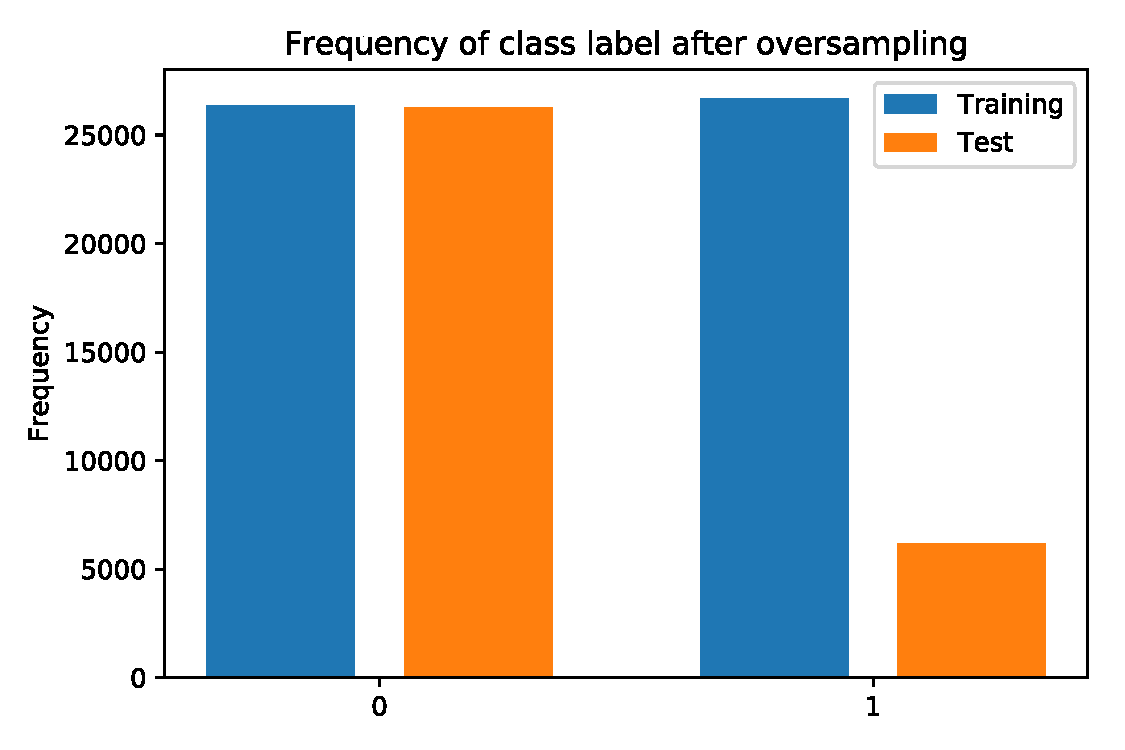
\includegraphics[width=0.7\textwidth]{pdf/oversampled.pdf}
%%\end{center}
%%\end{frame}
%%------------------------------------------------
%%\begin{frame}
%%\frametitle{Konfusionsmatrix nach Oversampling (Decision Tree)}
%%\begin{columns}[c] % The "c" option specifies centered vertical alignment while the "t" option is used for top vertical alignment
%%
%%\column{.5\textwidth} % Left column and width
%%\begin{tiny}
%%\begin{itemize}
%%\item  \textbf{erzielter Umsatz:} 11520.00 \euro{}
%%\item \textbf{Umsatzsteigerung:}	34.76 \% 
%%\item \textbf{Accuracy:} 75.23 \%
%%\end{itemize}
%%\end{tiny}
%%
%%\begin{figure}
%%\begin{center}
%%\includegraphics[width=.8\textwidth]{pdf/confusion2.pdf}
%%\end{center}
%%%\caption{Konfusionsmatrix nach Oversampling}
%%\end{figure}
%%
%%
%%\column{.5\textwidth} % Right column and width
%%\begin{center}
%%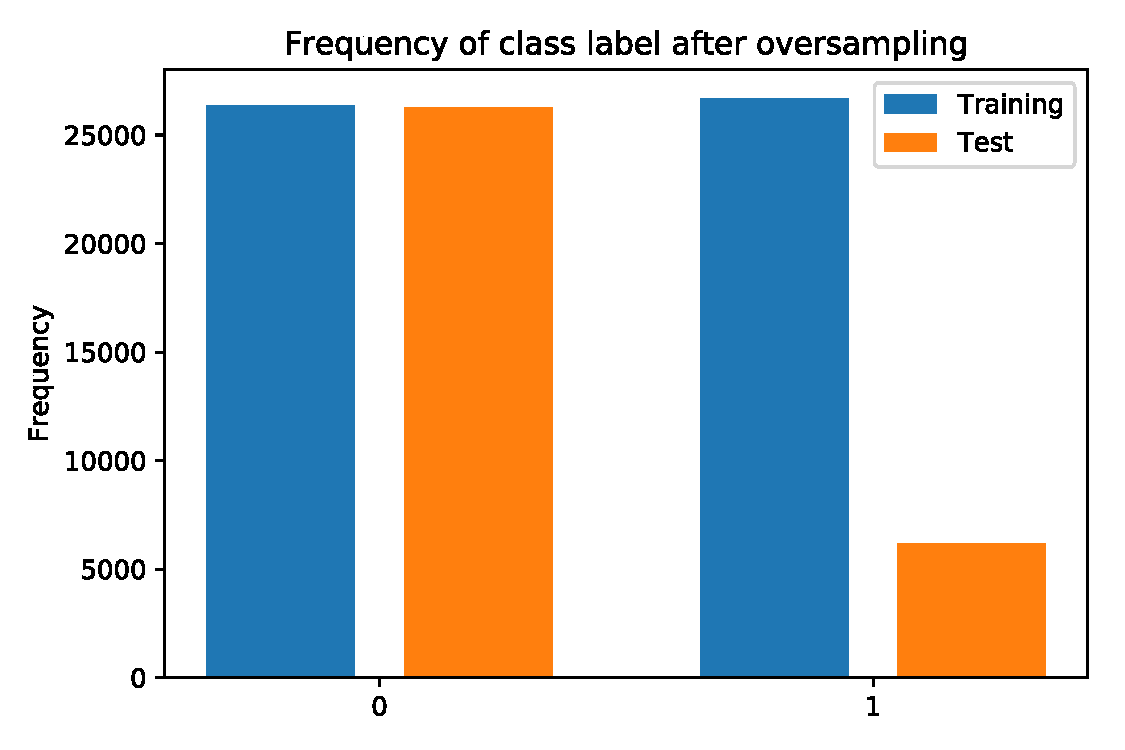
\includegraphics[width=.8\textwidth]{pdf/oversampled.pdf}
%%\end{center}
%%\end{columns}
%%\end{frame}
%
%
%%------------------------------------------------
%
%%\begin{frame}
%%\frametitle{Konfusionsmatrix nach Oversampling (Decision Tree)}
%%\begin{footnotesize}
%%\begin{itemize}
%%\item  \textbf{erzielter Umsatz:} 11520.00 \euro{}
%%\item \textbf{Umsatzsteigerung:}	25.79 \% 
%%\item \textbf{Accuracy:} 75.23 \%
%%\end{itemize}
%%\end{footnotesize}
%%
%%\begin{figure}
%%\begin{center}
%%\includegraphics[width=.5\textwidth]{pdf/confusion2.pdf}
%%\end{center}
%%%\caption{Konfusionsmatrix nach Oversampling}
%%\end{figure}
%%\end{frame}
%%------------------------------------------------
%%\begin{frame}
%%\frametitle{Backward Feature Elimination und Zeitmessung}
%%\begin{figure}
%%\begin{center}
%%\includegraphics[width=1.0\textwidth]{pdf/backwardSpark.pdf}
%%\end{center}
%%%\caption{Konfusionsmatrix Naiver Run}
%%\end{figure}
%%\end{frame}
%%
%%%------------------------------------------------
%%\begin{frame}
%%\frametitle{Zusammenfassung der Ergebnisse}
%%\begin{table}
%%\begin{tabular}{l c c}
%%\toprule
%%\textbf{Klassifikator} & \textbf{Umsatz} & \textbf{Steigerung}\\
%%\midrule
%%Ohne Optimierung & 8548.50 \euro{} & - \\
%%Decision Tree Naiv & 8552.00 \euro{} & 0.04 \%\\
%%Decision Tree Oversampling  & 11667.50 \euro{} & 36.49 \% \\
%%Random Forest Oversampling  & 11709.50 \euro{} &  36.98 \% \\
%%Optimaler Klassifikator  & 39388.50 \euro{} &  -\\
%%\bottomrule
%%\end{tabular}
%%%\caption{Ergebnisse}
%%\end{table}
%%\end{frame}
%
%
%------------------------------------------------

\begin{frame}
\frametitle{Literaturverzeichnis}
\begin{scriptsize}
\begin{thebibliography}{1}
\bibitem{1} Deep Learning, Ian Goodfellow and Yoshua Bengio and Aaron Courville, 2016
\bibitem{2} Convolutional neural networks: an overview and application in radiology, Yamashita, 2018
\bibitem{3} Script: Einführung in tiefe Lernverfahren - Faltungsnetzwerke,\\ Prof. Joachim Denzler
\bibitem{4} \url{https://towardsdatascience.com/a-comprehensive-guide-to-convolutional-neural-networks\\-the-eli5-way-3bd2b1164a53}
\bibitem{5} \url{https://aishack.in/tutorials/image-convolution-examples/}
\end{thebibliography}
\end{scriptsize}

\end{frame}

%------------------------------------------------



%----------------------------------------------------------------------------------------

\end{document} 